\documentclass{beamer}
\usepackage{beamerthemeshadow}
\usepackage{graphicx}
\usepackage{color}
\usepackage[utf8]{inputenc}
\usepackage{hyperref}
\usepackage[flushleft]{threeparttable}
\usepackage[english,serbianc]{babel}
\definecolor{beamer@darkred}{rgb}{0.85,0.1,0.1}
\setbeamercolor{structure}{fg=beamer@darkred}

\def\d{{\fontencoding{T1}\selectfont\dj}}
\def\D{{\fontencoding{T1}\selectfont\DJ}}

\title{Лични подаци на интернету}
\author{Давид Живковић}
\institute{Математички факултет\\Универзитет у Београду}
\date{
	\footnotesize{Београд 2020}
}

\begin{document}
\begin{frame}
	\thispagestyle{empty}
	\titlepage
\end{frame}

\addtocounter{framenumber}{-1}


\begin{frame}
	\frametitle{Садржај} 
	\tableofcontents[hidesubsections] 
\end{frame}


\section{Увод}

\begin{frame}[fragile]\frametitle{Шта су лични подаци на интернету ?}
	\begin{itemize}	
		\item \textbf{Лични подаци} су сви они подаци који се односе на особу, а на основу којих се она може идентификовати
		\item Сви подаци које ми остављамо се називају \textbf{дигитални отисак}, који даје врло прецизне информације о нама
		\item Своје „бесплатне” услуге компаније наплаћују корисницима тако што им заузврат траже све више личних података
		\item Те информације углавном користе како би нам доставили што прецизнији саджај, како би могли утицати на нас 
		
		
	\end{itemize}
\end{frame}


\subsection{Како све остављамо личне податке на интернету}

\begin{frame}[fragile]\frametitle{Како све остављамо личне податке на интернету}
	\begin{itemize}	
		\item \textbf{Сајтови и онлајн куповина}
		\item \textbf{Друштвене мреже}
		\item \textbf{Сви уређаји које користимо како бисмо приступили интернету}
		\item „\textbf{Лајкови}“
		
	\end{itemize}
\end{frame}


\subsection{}

\begin{frame}[fragile]\frametitle{Лајкови}
	\begin{itemize}	
		\item Лајкове ни мало не треба схватити олако, јер се успомоћ њих лако закључује о многим информацијама
		\begin{table}[h!]
\begin{center}

\begin{tabular}{|c|c|} \hline
\textbf{Податак} &\textbf{Проценат успешности}\\ \hline
Пол &93\% \\ \hline
Вера &82\%\\ \hline
Раса & 95\%\\ \hline
Пушач &73\% \\ \hline
Конзумира алкохол &70\% \\ \hline
Користи наркотике & 65\% \\ \hline
Сексуално опредељење &86\% \\ \hline
Политичко опредељење &85\% \\ \hline

\end{tabular}
\label{tab:tabela1}
\end{center}
\end{table}

	\end{itemize}
\end{frame}

\section{Врсте личних података}

\begin{frame}[fragile]\frametitle{Врсте личних података}
	\begin{itemize}	
		\item \textbf{Основни подаци}:
име и презиме особе, адреса становања, имејл адреса, фотографија, ИП адреса, итд.

 		\item \textbf{Подаци који служе за анализу и израду профила корисника}: радне способности, економско стање, лична интересовања, понашање, кретање итд.
 		\begin{figure}[h!]
\begin{center}
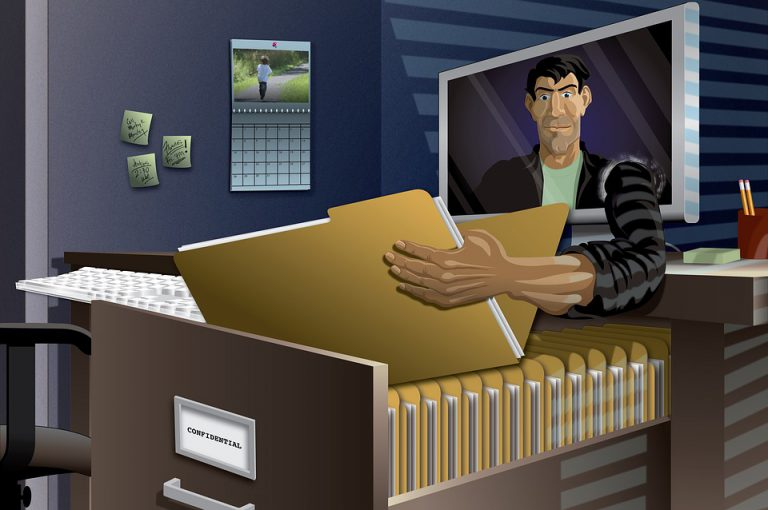
\includegraphics[scale=0.2]{slika.jpg}
\end{center}
\end{figure}
	\end{itemize}
\end{frame}

\begin{frame}[fragile]\frametitle{}
	\begin{itemize}	
		\item \textbf{Онлајн понашање особе}: подаци који се прикупљају посредством колачића 
		
\begin{figure}[h!]
\begin{center}
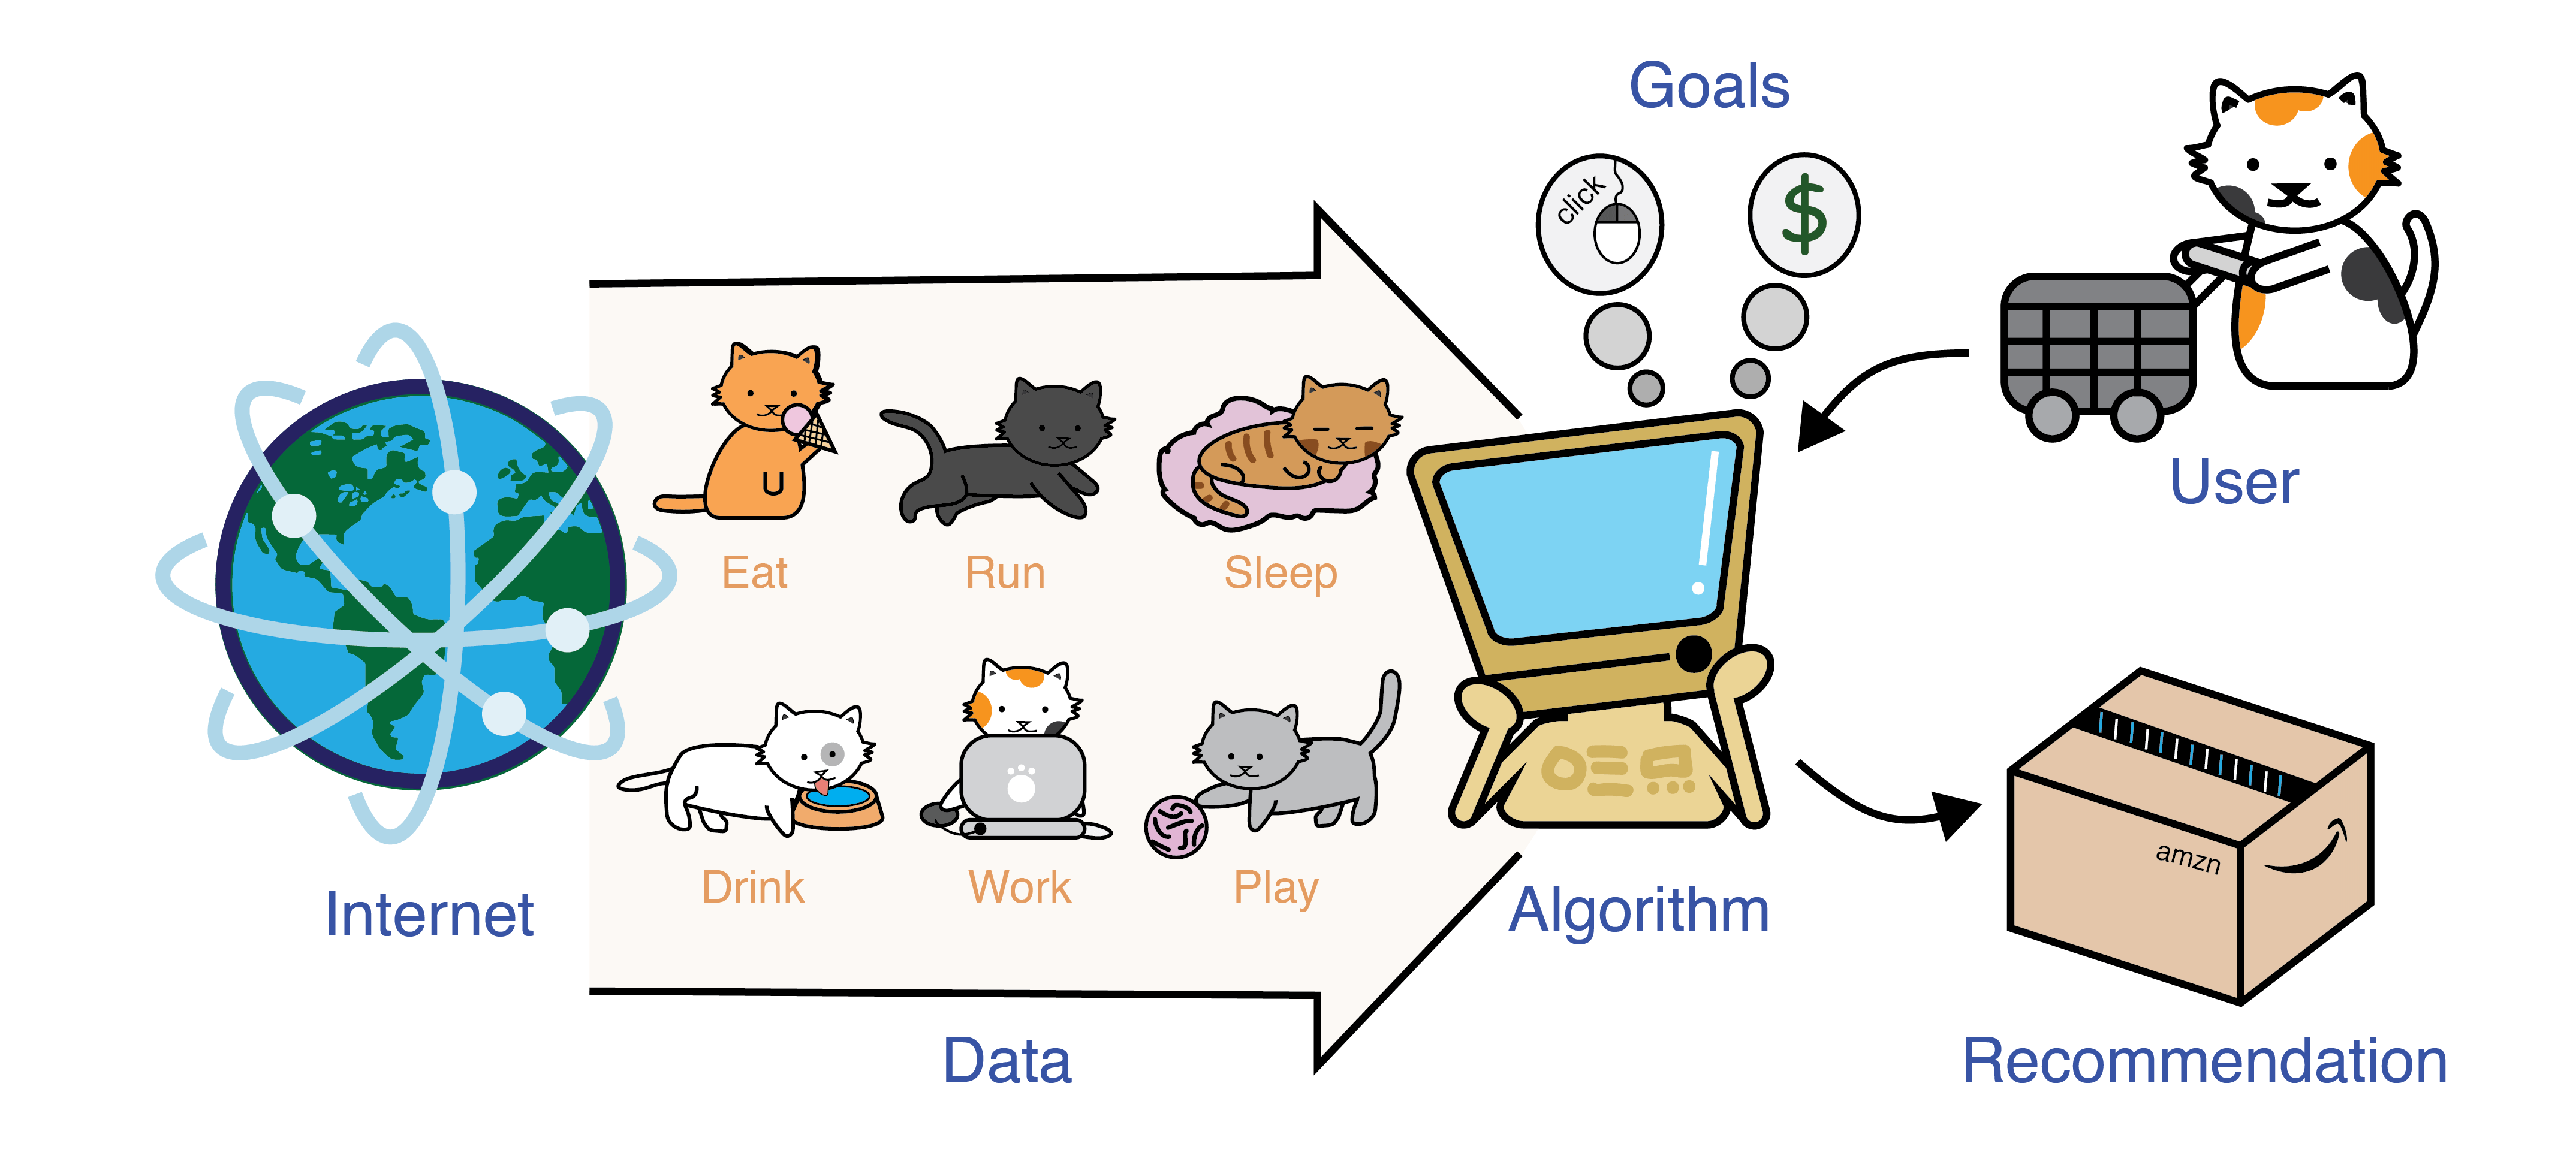
\includegraphics[scale=0.075]{slika2.jpg}
\caption{Проток наших података}
\end{center}
\end{figure}
		
	\end{itemize}
\end{frame}

\subsection{Врсте личних података на интернету}

\begin{frame}[fragile]\frametitle{Врсте личних података на интернету}
	\begin{itemize}	
	\item Лични подаци на интернету могу се груписати у три категорије:	
	\begin{itemize}
		\item\textbf{Активни дигитални трагови}: подаци (о себи или другима) које сами корисници остављају приликом коришћења интернета, обично свесно, мада не нужно и намерно  
		\item\textbf{Пасивни дигитални трагови}: подаци које корисници остављају на интернету приликом његовог коришћења, углавном несвесно
		\item\textbf{Подаци добијени анализом првих двеју категорија података}: помоћу алгоритама  (кроз процес профилисања), евентуално у комбинацији са другим изворима података				
	\end{itemize}
	\end{itemize}
\end{frame}

\subsection{Шерентинг}

\begin{frame}[fragile]\frametitle{Шерентинг}
	\begin{itemize}	
		\item Бројне личне информације могу бити скривене у фотографијама или видео-садржајима које постављамо на интернет 
		\item Родитељи често несвесно угрожавају право на приватност и безбедност сопствене деце
		\item Последњих година све се чешће говори о \textbf{шерентингу}
		
		\begin{figure}[h!]
\begin{center}
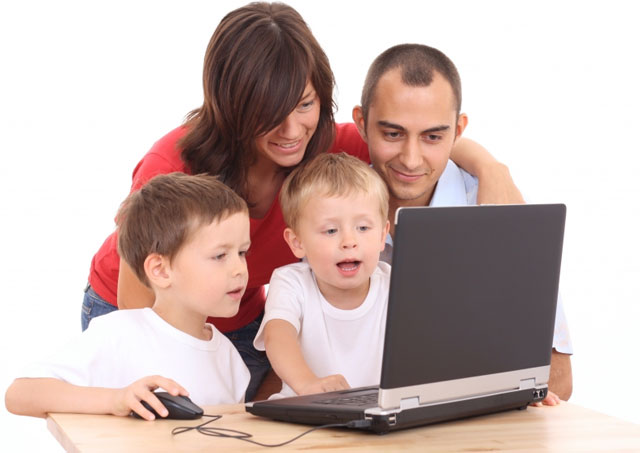
\includegraphics[scale=0.20]{dd.jpg}
\end{center}
\end{figure}
	\end{itemize}
\end{frame}


\section{Наша приватност на интернету}

\begin{frame}[fragile]\frametitle{Наша приватност}
	\begin{itemize}	
		\item Право на приватност и заштиту личних података јесте једно од основних права. Ово право односи се подједнако и на дигитално окружење
		\item Свака особа би требало да има могућност да, у зависности од ситуације и контекста, лично процени шта ће и са ким делити у свом \textbf{дигиталном окружењу}
		\item Свакo би требало да зна како и у које сврхе се користе њени подаци, ко их чува и колико дуго, ко све њима располаже, као и да може да затражи брисање или исправку нетачних података
	\end{itemize}
\end{frame}


\subsection{Како заштити личне податке и приватност на интернету}

\begin{frame}[fragile]\frametitle{Како заштити личне податке и приватност на интернету}
	\begin{itemize}	
		\item Дељење личних података само са блиским особама, не треба их делити са особама које не познајемо изван интернета
		\item Упознавање са \textbf{Условима коришћења} и \textbf{Политиком приватности} пре него што почнемо са коришћењем било које платформе, апликације или сервиса на интернету   
		\item Поштовање узрасног ограничења за коришћење сервиса, јер самом посетом било које веб-странице се остављају лични подаци на њој	
	\end{itemize}
\end{frame}


\section{Како заштити податке детета на интернету}

\begin{frame}[fragile]\frametitle{Подаци деце на интернету}
	\begin{itemize}	
		\item Велики број веб-сајтова и апликација траже од корисника да приликом отварања профила наведе свој \textbf{узраст}. На овим сервисима прописана је доња узрасна граница за њихово коришћење
		
		\item Како би заштитили корисника, али и себе (избегли кршење закона), веб-сајтови се обавезују да ће обрисати сваки профил који је креирала особа млађа од 13 година	
	\end{itemize}
\end{frame}


\subsection{Подаци деце на интернету}

\begin{frame}[fragile]\frametitle{Како заштити податке детета на интернету}
	
\begin{itemize}
	\item Уколико дете приликом отварања профила на неком сервису или друштвеној мрежи наведе да је старије него што јесте, може се десити да:
	\begin{itemize}
		\item Буде изложено садржајима који су неприкладни за његов узраст (узнемирујући, насилни или експлицитни)
		\item Изгуби додатне заштите и поставке приватности које се односе на узраст млађи од наведеног
		\item Лични профил детета, као и сав садржај на њему буду обрисани; осим тога, може му бити онемогућено да отвори лични профил чак и онда када достигне прописани узраст
\end{itemize}
	\item Због свега наведеног увек треба мотрити на понашање деце на интернету и не треба објављивати ништа што може превремено угрозити њихову приватност	
	\end{itemize}
	
\end{frame}


\section{Закључак}

\begin{frame}[fragile]\frametitle{Закључак}
	\begin{itemize}	
		\item На основу свега наведеног тешко је не забринути се за своју приватност и колико ја она до сад била компромитована
		\item Кад год желимо да приступимо интернету ми одајемо огромну количину својих личних података, а да о томе нисмо ни свесни
		\item Једино на шта можемо утицати је то да не дозволимо да се нама, као кориснику модерних технологија, не манипулише информацијама које смо им сами дали
	\end{itemize}
	
\end{frame}

\subsubsection{}

\begin{frame}[fragile]\frametitle{Закључак}
	\begin{itemize}
	\item 

		\begin{figure}[h!]
\begin{center}

\includegraphics[scale=0.25]{Untitled1.png}
\end{center}
\end{figure}


\end{itemize}

\end{frame}
	

\end{document}